% !TEX root = ../main.tex
\section{Figures and Tables}

\begin{figure}[h!]
    \centering
    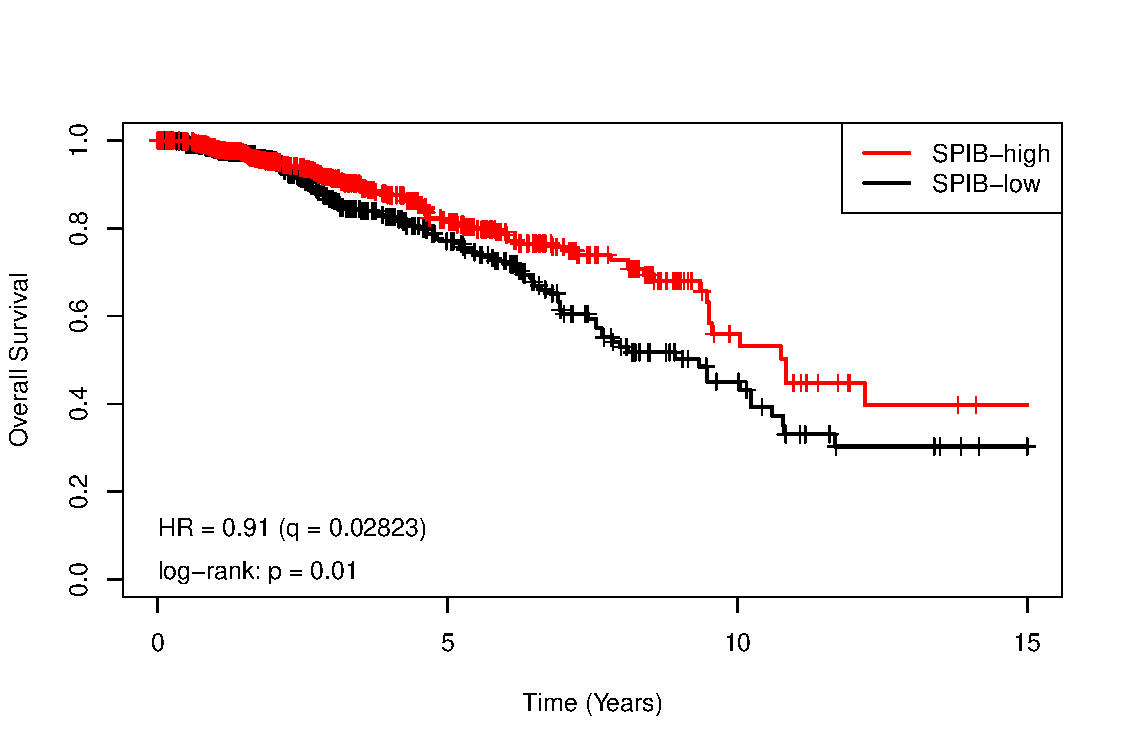
\includegraphics[scale=0.70]{figures/km_plot.pdf}
    \caption{Survival of SPIB-high and SPIB-low breast cancer patients. Data from the TCGA BRCA dataset \cite{Ciriello2015, Goldman2018}.}
    \label{km_plot}
\end{figure} 

\begin{figure}[h!]
    \centering
    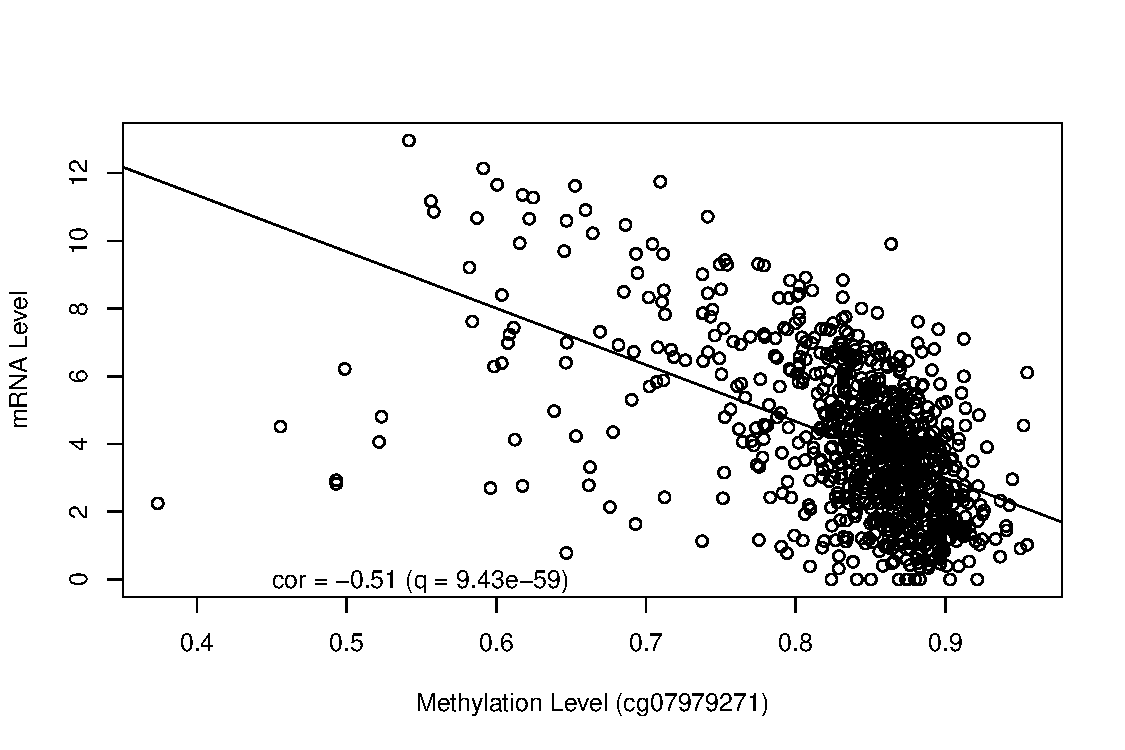
\includegraphics[scale=0.75]{figures/methylation.pdf}
    \caption{Scatter plot of SPIB methlyation vs mRNA expression values. Spearman correlation shown. Data from the TCGA BRCA dataset \cite{Ciriello2015, Goldman2018}.}
    \label{methylation}
\end{figure} 

\begin{figure}[h!]
    \centering
    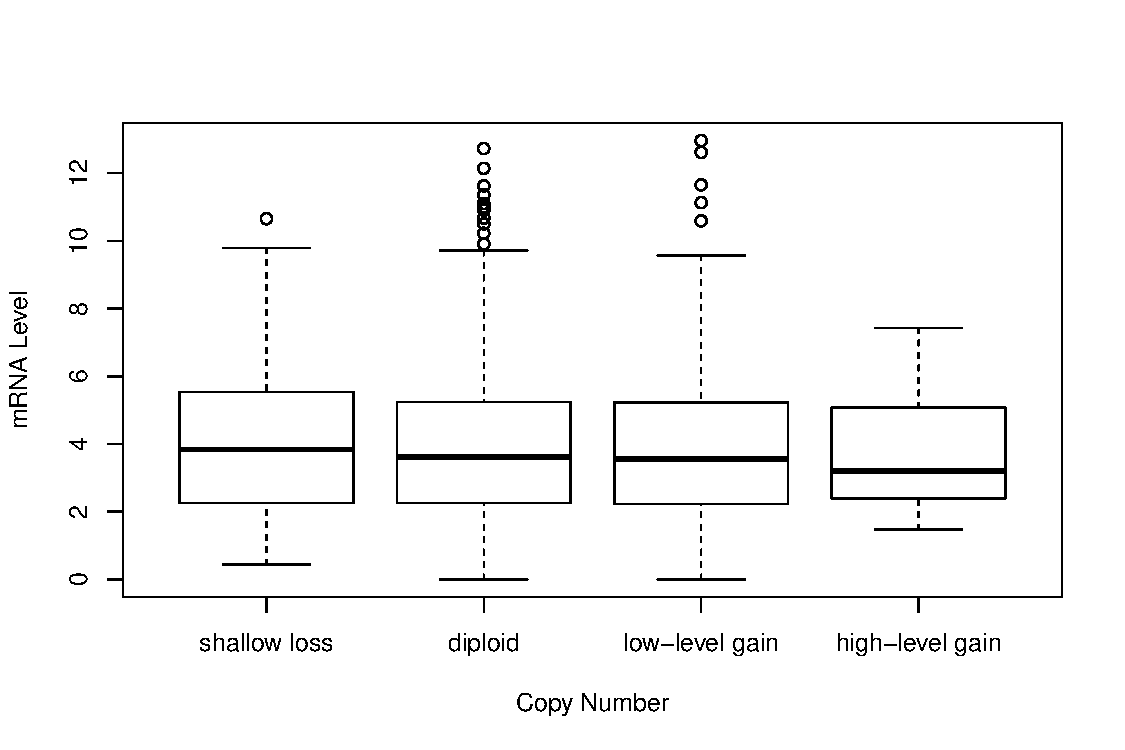
\includegraphics[scale=0.75]{figures/cnv.pdf}
    \caption{mRNA expression of SPIB compared under different copy number alteration levels. Data from the TCGA BRCA dataset \cite{Ciriello2015, Goldman2018}.}
    \label{cnv}
\end{figure} 

\begin{table}[!p]
    \centering
    \caption{Methylation Sites}
    \begin{center}
    \begin{tabular}{l|lllll}
        CpG & cor & p-value & q-value & Mean (SPIB-High) & Mean (SPIB-Low) \\ \hline
        cg07979271 & $-0.514$ & $5.55 \cdot 10^{-60}$ & $9.43 \cdot 10^{-59}$ & $0.816$ & $0.864$\\ 
        cg13403724 & $0.288 $& $3.80 \cdot 10^{-18}$ & $3.23 \cdot 10^{-17}$ & $0.248$ & $0.206$\\ 
        cg17774764 & $-0.281$ & $3.07 \cdot 10^{-17}$ & $1.74 \cdot 10^{-16}$ & $0.737$ & $0.775$\\ 
        cg03763616 & $-0.277$ & $7.68 \cdot 10^{-17}$ & $3.26 \cdot 10^{-16}$ & $0.832$ & $0.859$\\ 
        cg19387862 & $0.272$& $2.70 \cdot 10^{-16}$ & $9.20 \cdot 10^{-16}$ & $0.191$ & $0.168$\\ 
        cg15690347 & $0.266$& $1.25 \cdot 10^{-15}$ & $3.54 \cdot 10^{-15}$ & $0.383$ & $0.301$\\ 
        cg08201854 & $0.265$& $1.87 \cdot 10^{-15}$ & $4.55 \cdot 10^{-15}$ & $0.26$ & $0.226$\\ 
        cg15007959 & $0.263$& $3.08 \cdot 10^{-15}$ & $6.55 \cdot 10^{-15}$ & $0.253$ & $0.203$\\ 
        cg18254819 & $0.246$& $1.53 \cdot 10^{-13}$ & $2.90 \cdot 10^{-13}$ & $0.235$ & $0.212$\\ 
        cg24092179 & $0.228$& $1.00 \cdot 10^{-11}$ & $1.71 \cdot 10^{-11}$ & $0.271$ & $0.244$\\ 
        cg22268231 & $-0.147$ & $1.22 \cdot 10^{-05}$ & $1.88 \cdot 10^{-05}$ & $0.45$ & $0.487$\\ 
        cg06512885 & $-0.133$ & $7.89 \cdot 10^{-05}$ & $0.000112$ & $0.875$ & $0.881$\\ 
        cg26522743 & $-0.0968$ & $0.0042$ & $0.00549$ & $0.394$ & $0.424$\\ 
        cg21152077 & $0.0921$ & $0.00653$ & $0.00792$ & $0.464$ & $0.448$\\ 
        cg13918544 & $0.0845$ & $0.0125$ & $0.0141$ & $0.132$ & $0.143$\\ 
        cg22745102 & $0.0705$ & $0.0372$ & $0.0396$ & $0.469$ & $0.462$\\ 
        cg04508467 & $2.02 \cdot 10^{-05}$ & $1$ & $1$ & $0.696$ & $0.686$\\ \hline
    \end{tabular}
    \end{center}
    Spearman correlation of methylation of CpG islands and the mRNA expression of SPIB.
    \label{meth_table}
\end{table} 
    